
\documentclass[a4paper,12pt]{article}

%%% Работа с русским языком
\usepackage{cmap}					% поиск в PDF
\usepackage{mathtext} 				% русские буквы в формулах
\usepackage[T2A]{fontenc}			% кодировка
\usepackage[utf8]{inputenc}			% кодировка исходного текста
\usepackage[english]{babel}	% локализация и переносы
\usepackage{indentfirst}
\frenchspacing
\usepackage{amsmath}

\newcommand{\bz}{\mathbf{z}}
\newcommand{\bx}{\mathbf{x}}
\newcommand{\by}{\mathbf{y}}
\newcommand{\bv}{\mathbf{v}}
\newcommand{\bw}{\mathbf{w}}
\newcommand{\ba}{\mathbf{a}}
\newcommand{\bb}{\mathbf{b}}
\newcommand{\bp}{\mathbf{p}}
\newcommand{\bq}{\mathbf{q}}
\newcommand{\bt}{\mathbf{t}}
\newcommand{\bu}{\mathbf{u}}
\newcommand{\bT}{\mathbf{T}}
\newcommand{\bX}{\mathbf{X}}
\newcommand{\bZ}{\mathbf{Z}}
\newcommand{\bS}{\mathbf{S}}
\newcommand{\bH}{\mathbf{H}}
\newcommand{\bW}{\mathbf{W}}
\newcommand{\bY}{\mathbf{Y}}
\newcommand{\bU}{\mathbf{U}}
\newcommand{\bQ}{\mathbf{Q}}
\newcommand{\bP}{\mathbf{P}}
\newcommand{\bA}{\mathbf{A}}
\newcommand{\bB}{\mathbf{B}}
\newcommand{\bC}{\mathbf{C}}
\newcommand{\bE}{\mathbf{E}}
\newcommand{\bF}{\mathbf{F}}
\newcommand{\bomega}{\boldsymbol{\omega}}
\newcommand{\btheta}{\boldsymbol{\theta}}
\newcommand{\bgamma}{\boldsymbol{\gamma}}
\newcommand{\bdelta}{\boldsymbol{\delta}}
%\newcommand{\bPsi}{\boldsymbol{\Psi}}
%\newcommand{\bpsi}{\boldsymbol{\psi}}
\newcommand{\bxi}{\boldsymbol{\xi}}
\newcommand{\bchi}{\boldsymbol{\chi}}
\newcommand{\bzeta}{\boldsymbol{\zeta}}
\newcommand{\blambda}{\boldsymbol{\lambda}}
\newcommand{\beps}{\boldsymbol{\varepsilon}}
\newcommand{\bZeta}{\boldsymbol{Z}}
% mathcal
\newcommand{\cX}{\mathcal{X}}
\newcommand{\cY}{\mathcal{Y}}
\newcommand{\cW}{\mathcal{W}}

\newcommand{\dH}{\mathbb{H}}
\newcommand{\dR}{\mathbb{R}}
% transpose
\newcommand{\T}{^{\mathsf{T}}}

\renewcommand{\epsilon}{\ensuremath{\varepsilon}}
%\renewcommand{\phi}{\ensuremath{\varphi}}
\renewcommand{\kappa}{\ensuremath{\varkappa}}
\renewcommand{\le}{\ensuremath{\leqslant}}
\renewcommand{\leq}{\ensuremath{\leqslant}}
\renewcommand{\ge}{\ensuremath{\geqslant}}
\renewcommand{\geq}{\ensuremath{\geqslant}}
\renewcommand{\emptyset}{\varnothing}

%%% Дополнительная работа с математикой
\usepackage{amsmath,amsfonts,amssymb,amsthm,mathtools} % AMS
\usepackage{icomma} % "Умная" запятая: $0,2$ --- число, $0, 2$ --- перечисление

%% Номера формул
%\mathtoolsset{showonlyrefs=true} % Показывать номера только у тех формул, на которые есть \eqref{} в тексте.
%\usepackage{leqno} % Нумереация формул слева

%% Свои команды
\DeclareMathOperator{\sgn}{\mathop{sgn}}

%% Перенос знаков в формулах (по Львовскому)
\newcommand*{\hm}[1]{#1\nobreak\discretionary{}
	{\hbox{$\mathsurround=0pt #1$}}{}}

%%% Работа с картинками
\usepackage{graphicx}  % Для вставки рисунков
\setlength\fboxsep{3pt} % Отступ рамки \fbox{} от рисунка
\setlength\fboxrule{1pt} % Толщина линий рамки \fbox{}
\usepackage{wrapfig} % Обтекание рисунков текстом

%%% Работа с таблицами
\usepackage{array,tabularx,tabulary,booktabs} % Дополнительная работа с таблицами
\usepackage{longtable}  % Длинные таблицы
\usepackage{multirow} % Слияние строк в таблице

%%% Теоремы
\theoremstyle{plain} % Это стиль по умолчанию, его можно не переопределять.
\newtheorem{theorem}{Теорема}[section]
\newtheorem{proposition}[theorem]{Утверждение}

\theoremstyle{definition} % "Определение"
\newtheorem{corollary}{Следствие}[theorem]
\newtheorem{problem}{Задача}[section]

\theoremstyle{remark} % "Примечание"
\newtheorem*{nonum}{Решение}

%%% Программирование
\usepackage{etoolbox} % логические операторы

%%% Страница
\usepackage{extsizes} % Возможность сделать 14-й шрифт
\usepackage{geometry} % Простой способ задавать поля
\geometry{top=25mm}
\geometry{bottom=35mm}
\geometry{left=35mm}
\geometry{right=20mm}
%
%\usepackage{fancyhdr} % Колонтитулы
% 	\pagestyle{fancy}
%\renewcommand{\headrulewidth}{0pt}  % Толщина линейки, отчеркивающей верхний колонтитул
% 	\lfoot{Нижний левый}
% 	\rfoot{Нижний правый}
% 	\rhead{Верхний правый}
% 	\chead{Верхний в центре}
% 	\lhead{Верхний левый}
%	\cfoot{Нижний в центре} % По умолчанию здесь номер страницы

\usepackage{setspace} % Интерлиньяж
%\onehalfspacing % Интерлиньяж 1.5
%\doublespacing % Интерлиньяж 2
%\singlespacing % Интерлиньяж 1

\usepackage{lastpage} % Узнать, сколько всего страниц в документе.

\usepackage{soul} % Модификаторы начертания

\usepackage{hyperref}
\usepackage[usenames,dvipsnames,svgnames,table,rgb]{xcolor}
\hypersetup{				% Гиперссылки
	unicode=true,           % русские буквы в раздела PDF
	pdftitle={Заголовок},   % Заголовок
	pdfauthor={Автор},      % Автор
	pdfsubject={Тема},      % Тема
	pdfcreator={Создатель}, % Создатель
	pdfproducer={Производитель}, % Производитель
	pdfkeywords={keyword1} {key2} {key3}, % Ключевые слова
	colorlinks=true,       	% false: ссылки в рамках; true: цветные ссылки
	linkcolor=red,          % внутренние ссылки
	citecolor=black,        % на библиографию
	filecolor=magenta,      % на файлы
	urlcolor=cyan           % на URL
}

\usepackage{csquotes} % Еще инструменты для ссылок

%\usepackage[style=authoryear,maxcitenames=2,backend=biber,sorting=nty]{biblatex}

\usepackage{multicol} % Несколько колонок

\usepackage{tikz} % Работа с графикой
\usepackage{pgfplots}
\usepackage{pgfplotstable}


\author{Boeva Galina, group М05-304а}
\title{\textbf{CCA to Normilizing Flows}}
\date{\today}

\begin{document}
\maketitle

\section*{Introduction}

When observations consist of multiple views or modalities of the same underlying source of variation, a learning algorithm should efficiently account for the complementary information to alleviate learning difficulty~\cite{chaudhuri2009consequences} and improve accuracy. A well-established method for two-view analysis is given by canonical correlation analysis (CCA)~\cite{hotelling1992relations}, a classical subspace learning technique that extracts the common information between
two multivariate random variables by projecting them onto a subspace. CCA, as a standard model for unsupervised two-view learning, has been used in a broad range of tasks such as dimensionality reduction, visualization and time series analysis~\cite{xia2014two}. А modified formulation of probabilistic CCA is presented, then this linear probabilistic layer is extended to an interpretable deep generative multi-view network. The proposed model captures the variations of the views by a shared latent representation, describing the common underlying sources of variation, i.e. the essence of multi-view data,
and a set of view-specific latent factors. 

\section*{Probabilistic CCA}
The probabilistic generative model for the graphical
model in Figure 1.1 is defined as:
\begin{equation}
\phi \sim \mathcal{N}(\boldsymbol{\mu}_0, \boldsymbol{I}_{d_0}), 0 < d_0 \leq \min(d_1, d_2)
\end{equation}

\begin{equation}
\boldsymbol{z_1} | \phi \sim \mathcal{N}(\boldsymbol{W_1} \phi + \boldsymbol{\mu}_{\epsilon_1}, \boldsymbol{\Psi}_1), \boldsymbol{W_1} \in \mathbb{R}^{d_1 \times d_0}, \boldsymbol{\Psi}_1 \succeq 0
\end{equation}

\begin{equation}
\boldsymbol{z_2} | \phi \sim \mathcal{N}(\boldsymbol{W_2} \phi + \boldsymbol{\mu}_{\epsilon_2}, \boldsymbol{\Psi}_2), \boldsymbol{W_2} \in \mathbb{R}^{d_2 \times d_0}, \boldsymbol{\Psi}_2 \succeq 0
\end{equation}
where $\phi$ is the shared latent representation. The maximum likelihood estimate of the parameters of this model can be expressed in terms of the canonical correlation directions as:

\[\hat{\boldsymbol{W}}_1 = \boldsymbol{\Sigma}_{11}\boldsymbol{U}_1 \boldsymbol{M}, \hat{\boldsymbol{W}}_2 = \boldsymbol{\Sigma}_{22}\boldsymbol{U}_2 \boldsymbol{M}\]
 
\[\hat{\boldsymbol{\Psi}}_1 = \boldsymbol{\Sigma}_{11} - \hat{\boldsymbol{W}}_1\hat{\boldsymbol{W}}_1^T, \hat{\boldsymbol{\Psi}}_2 = \boldsymbol{\Sigma}_{22} - \hat{\boldsymbol{W}}_2\hat{\boldsymbol{W}}_2^T\] 

\[\hat{\boldsymbol{\mu}}_{\epsilon_1} = \boldsymbol{\mu}_1 - \hat{\boldsymbol{W}}_1 \boldsymbol{\mu}_0, \hat{\boldsymbol{\mu}}_{\epsilon_2} = \boldsymbol{\mu}_2 - \hat{\boldsymbol{W}}_2 \boldsymbol{\mu}_0\]
where $\boldsymbol{M} = \boldsymbol{P}^{1/2}_{d_0} \boldsymbol{R}$ is the square root of matrix $\boldsymbol{P}_{d_0}$ and $\boldsymbol{R}$ is an arbitrary rotation matrix and the residual errors terms can be defined as $\boldsymbol{\epsilon}_1 := \boldsymbol{z}_1 - \boldsymbol{W}_1 \phi$
and  $\boldsymbol{\epsilon}_2 := \boldsymbol{z}_2 - \boldsymbol{W}_2 \phi$. This probabilistic graphical model induces conditional
independence of $\boldsymbol{z}_1$ and $\boldsymbol{z}_2$ given $\phi$. The parameter $\boldsymbol{\mu}_0$ is not identifiable by
maximum likelihood. 

In contrast to the results in~\cite{bach2005probabilistic}, where  $\boldsymbol{\mu}_0 = 0$, here we introduce $\boldsymbol{\mu}_0$  as an extra degree of freedom.

\begin{figure}
    \centering
    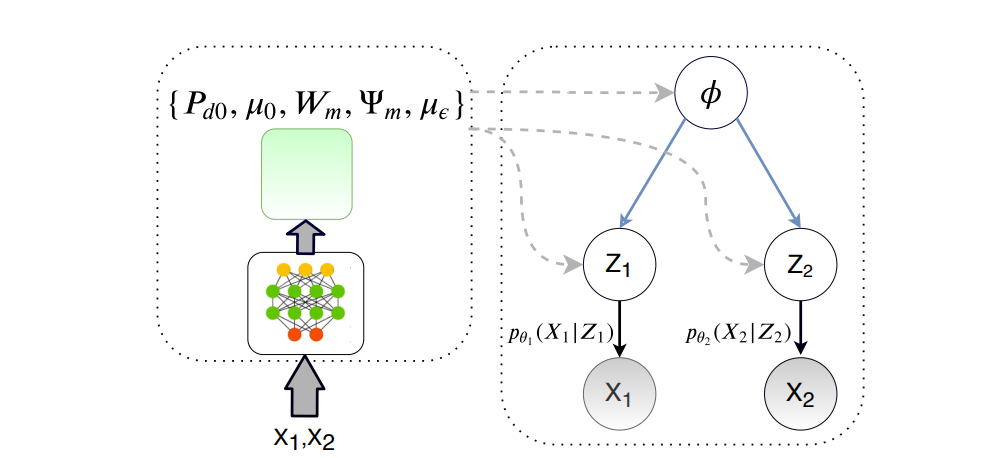
\includegraphics[width=0.5\textwidth]{images/essay3.png}
    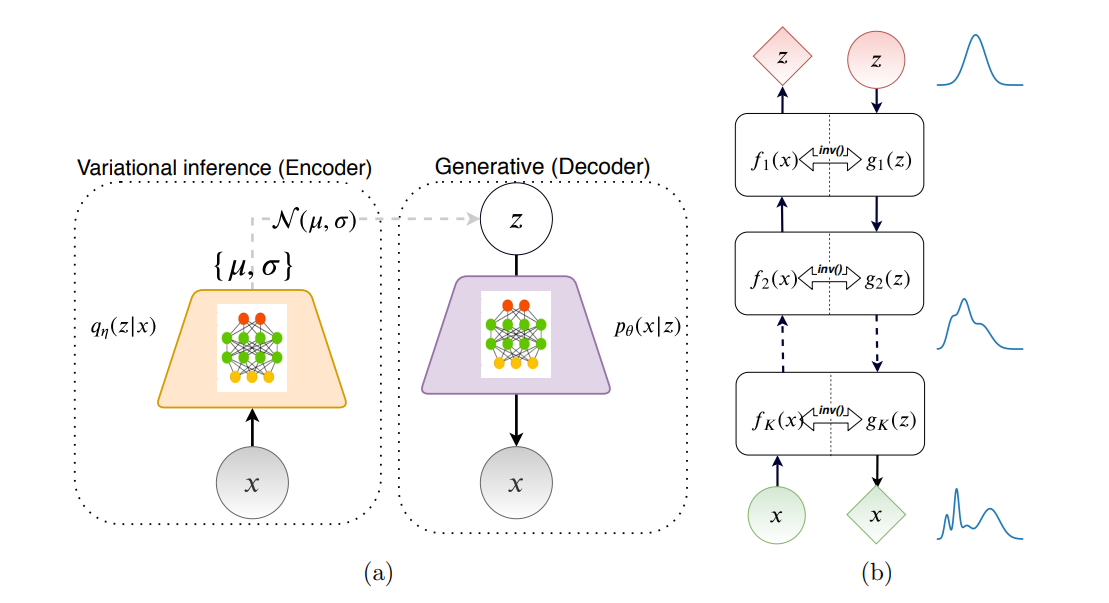
\includegraphics[width=0.49\textwidth]{images/essay4.png}
    \caption{1. Graphical representation of the deep probabilistic CCA model, where the blue edges belong to latent linear probabilistic CCA model and the black edges represent the deep nonlinear observation networks (decoders) $p_{\theta_m} (\textbf{x}_m|\textbf{z}_m) = g_m(\textbf{z}_m; \theta_m)$. Shaded nodes denotes observed views and dashed line represent the stochastic samples drawn from the approximate posteriors. 2. Schematic representation of (a) a vanilla Variational Auto-Encoder model, and (b) a Normalizing Flow model.}
    \label{fig:enter-label}
\end{figure}
\section*{Normalizing Flows}

Another line of work~\cite{karami2020advances} that has received a large amount of interest recently is to directly estimate the distribution of the data by normalizing flows. The normalizing flow is a chain of smooth and invertible transformations (bijections) to construct a complex probability density by transforming a simple base density, such as a standard normal distribution, exploiting the change of variable formula.
Given a random variable $\boldsymbol{z} \sim p(\boldsymbol{z})$ and an invertible and differentiable mapping $g: \mathbb{R}^n \rightarrow \mathbb{R}^n$, with inverse mapping $f = g^{-1}$, the probability density function of the transformed variable $\boldsymbol{x} = g(\boldsymbol{z})$ can be described by the change of variable formula as
\begin{equation} 
p(\boldsymbol{x}) = p(\boldsymbol{z}) \left| \det \boldsymbol{J}_g \right|^{-1} = p(f(\boldsymbol{x})) \left| \det \boldsymbol{J}_f \right| 
\end{equation}
This formula provides a framework for probabilistic generative modeling.

Authors of the NICE~\cite{dinh2014nice} model proposed using the following family of transformations for $g_\theta$:

\[
\boldsymbol{x} = g_\theta(\boldsymbol{z}) = \begin{cases}
\boldsymbol{x}_{1:d} = \boldsymbol{z}_{1:d} \\
\boldsymbol{x}_{d+1:n} = \boldsymbol{z}_{d+1:n} + m_\theta(\boldsymbol{z}_{1:d}),
\end{cases}
\]

where $1 < d < n$, and $m_\theta$ is an arbitrary neural network with $d$ inputs and $n-d$ outputs. This transformation is called additive coupling.

The inverse transformation is computed with the same ease, and the Jacobian is equal to $1$. That is,
\[
p_{\boldsymbol{x}}(\boldsymbol{x}) = p_{\boldsymbol{z}}(g^{-1}(\boldsymbol{x})),
\]
which is a fairly strong constraint on the model.

Furthermore, since
\[
\boldsymbol{x}_{1:d} = \boldsymbol{z}_{1:d},
\]
the first $d$ channels of the vector $\boldsymbol{x}$ coincide with the coordinates of the normal noise $\boldsymbol{z}$, meaning that these channels of $\boldsymbol{x}$ are not modeled. Due to this, the expressive power of the NICE model was relatively low.

Later, the authors of NICE proposed using fixed permutations of features/channels $\boldsymbol{x}$ between layers of normalizing flows, which became the basis for the work on RealNVP. Using permutations allows all output channels to be affected by the transformation $g_\theta(\boldsymbol{z})$; moreover, the gradient of the permutation is easily computed.

\[
\boldsymbol{x} = g_\theta(\boldsymbol{z}) = \begin{cases}
\boldsymbol{x}_{1:d} = \boldsymbol{z}_{1:d} \\
\boldsymbol{x}_{d+1:n} = \exp(s_\theta(\boldsymbol{z}_{1:d})) \odot \boldsymbol{z}_{d+1:n} + m_\theta(\boldsymbol{z}_{1:d}),
\end{cases}
\]

where $\odot$ denotes element-wise multiplication, and $s_\theta$ is a neural network that can be arbitrary but is usually chosen to have the same architecture as $m_\theta$. This transformation is called affine coupling.

The resulting mapping is also easily inverted, and its Jacobian is equal to:

\[
\det(\boldsymbol{J}_{g^{-1}}) = \exp \left( \sum_{i=d+1}^n (s_\theta(\boldsymbol{z}_{1:d}))_i \right)
\]

Note that, as in the case of additive coupling, a significant portion of the channels remains unchanged when using affine coupling. To ensure that the transformation $g_\theta(\boldsymbol{x})$ models the distribution of $\boldsymbol{x}$ in all channels, different subsets of $d$ channels are left unchanged on different layers.
 

\section*{Conclusion} 

This work presents a modified formulation of probabilistic canonical correlation analysis (CCA) and extends it to an interpretable deep generative multi-view network. Additionally, the integration of normalizing flows enhances the model's ability to estimate complex data distributions, providing a robust framework for probabilistic generative modeling.


\bibliography{biblio}
\bibliographystyle{unsrt}
\end{document}
